\begin{frame}[plain]{Conjunto de datos: NF-UNSW-NB15-v3}

\begin{tikzpicture}

% Nodo de la tabla centrado
\node (tabla) at (0,0) {
\scriptsize
\adjustbox{width=0.95\textwidth}{
\begin{tabular}{|c|c|c|c|c|c|c|c|}
\hline
\textbf{\#} & \cellcolor{headerblue} Dur & \cellcolor{headerblue} Proto & \cellcolor{headerblue} SBytes & \cellcolor{headerblue} DBytes & \cellcolor{headerblue} $\cdots$ & \cellcolor{labelbeige} Label & \cellcolor{labelbeige} Attack \\
\hline
0 & 4,7 & TCP & 102 & 300 & $\cdots$ & \cellcolor{white}0 & \cellcolor{white}Benign \\
1 & 7,3 & UDP & 215 & 540 & $\cdots$ & \cellcolor{lightred}1 & \cellcolor{Fuzzers}Fuzzers \\
2 & 0,9 & TCP & 98 & 188 & $\cdots$ & \cellcolor{white}0 & \cellcolor{white}Benign \\
3 & 3,6 & TCP & 155 & 222 & $\cdots$ & \cellcolor{lightred}1 & \cellcolor{Generic}Generic \\
4 & 6,4 & UDP & 300 & 310 & $\cdots$ & \cellcolor{lightred}1 & \cellcolor{Exploits}Exploits \\
5 & 1,8 & ICMP & 65 & 120 & $\cdots$ & \cellcolor{white}0 & \cellcolor{white}Benign \\
6 & 5,5 & TCP & 180 & 390 & $\cdots$ & \cellcolor{lightred}1 & \cellcolor{Backdoor}Backdoor \\
7 & 2,9 & TCP & 143 & 305 & $\cdots$ & \cellcolor{lightred}1 & \cellcolor{DoS}DoS \\
8 & 9,1 & UDP & 260 & 470 & $\cdots$ & \cellcolor{white}0 & \cellcolor{white}Benign \\
9 & 1,2 & TCP & 97 & 190 & $\cdots$ & \cellcolor{white}0 & \cellcolor{white}Benign \\
10 & 4,3 & ICMP & 120 & 240 & $\cdots$ & \cellcolor{lightred}1 & \cellcolor{Exploits}Exploits \\
\textbf{$\vdots$} & $\vdots$ & $\vdots$ & $\vdots$ & $\vdots$ & $\vdots$ & $\vdots$ & $\vdots$ \\
\textbf{2\,365\,424} & 3,2 & TCP & 245 & 510 & $\cdots$ & \cellcolor{lightred}1 & \cellcolor{DoS}DoS \\
\hline
\end{tabular}}
};

% === Llaves ajustadas y divididas ===
% Atributos: columnas 2 a 6
\draw[decorate,decoration={brace,amplitude=5pt},thick]
($(tabla.north west)+(1.8, 0.05)$) -- ($(tabla.north west)+(7.55,0.05)$)
node[midway,yshift=0.42cm]{\scriptsize \textbf{Atributos (53)}};

% Etiquetas: columnas 7 y 8
\draw[decorate,decoration={brace,amplitude=5pt},thick]
($(tabla.north west)+(7.65,0.05)$) -- ($(tabla.north west)+(10.4,0.05)$)
node[midway,yshift=0.42cm]{\scriptsize \textbf{Etiquetas (2)}};

% Llave lateral izquierda
\draw[decorate,decoration={brace,amplitude=5pt,mirror},thick]
($(tabla.north west)+(0,-0.1)$) -- ($(tabla.south west)+(0,0.1)$)
node[midway,xshift=-0.42cm,rotate=90]{\scriptsize \textbf{Conexiones}};


\end{tikzpicture}

\end{frame}




\begin{frame}[plain]{Número de muestras por clase del conjunto de datos}

\begin{tikzpicture}

% === Tabla principal (NO SE MUEVE) ===
\node (tabla) at (0,0) {
\scriptsize
\adjustbox{width=0.95\textwidth}{
\begin{tabular}{|c|c|c|c|c|c|c|c|}
\hline
\textbf{\#} & \cellcolor{headerblue} Dur & \cellcolor{headerblue} Proto & \cellcolor{headerblue} SBytes & \cellcolor{headerblue} DBytes & \cellcolor{headerblue} $\cdots$ & \cellcolor{labelbeige} Label & \cellcolor{labelbeige} Attack \\
\hline
\hline
0 & 4,7 & TCP & 102 & 300 & $\cdots$ & \cellcolor{white}0 & \cellcolor{white}Benign \\
1 & 7,3 & UDP & 215 & 540 & $\cdots$ & \cellcolor{lightred}1 & \cellcolor{Fuzzers}Fuzzers \\
2 & 0,9 & TCP & 98 & 188 & $\cdots$ & \cellcolor{white}0 & \cellcolor{white}Benign \\
3 & 3,6 & TCP & 155 & 222 & $\cdots$ & \cellcolor{lightred}1 & \cellcolor{Generic}Generic \\
4 & 6,4 & UDP & 300 & 310 & $\cdots$ & \cellcolor{lightred}1 & \cellcolor{Exploits}Exploits \\
5 & 1,8 & ICMP & 65 & 120 & $\cdots$ & \cellcolor{white}0 & \cellcolor{white}Benign \\
6 & 5,5 & TCP & 180 & 390 & $\cdots$ & \cellcolor{lightred}1 & \cellcolor{Backdoor}Backdoor \\
7 & 2,9 & TCP & 143 & 305 & $\cdots$ & \cellcolor{lightred}1 & \cellcolor{DoS}DoS \\
8 & 9,1 & UDP & 260 & 470 & $\cdots$ & \cellcolor{white}0 & \cellcolor{white}Benign \\
9 & 1,2 & TCP & 97 & 190 & $\cdots$ & \cellcolor{white}0 & \cellcolor{white}Benign \\
10 & 4,3 & ICMP & 120 & 240 & $\cdots$ & \cellcolor{lightred}1 & \cellcolor{Exploits}Exploits \\
\textbf{$\vdots$} & $\vdots$ & $\vdots$ & $\vdots$ & $\vdots$ & $\vdots$ & $\vdots$ & $\vdots$ \\
\textbf{2\,365\,424} & 3,2 & TCP & 245 & 510 & $\cdots$ & \cellcolor{lightred}1 & \cellcolor{DoS}DoS \\
\hline
\end{tabular}}
};


% === Llaves ajustadas y divididas ===
% Atributos: columnas 2 a 6
\draw[decorate,decoration={brace,amplitude=5pt},thick]
($(tabla.north west)+(1.8, 0.05)$) -- ($(tabla.north west)+(7.55,0.05)$)
node[midway,yshift=0.42cm]{\scriptsize \textbf{Atributos (53)}};

% Etiquetas: columnas 7 y 8
\draw[decorate,decoration={brace,amplitude=5pt},thick]
($(tabla.north west)+(7.65,0.05)$) -- ($(tabla.north west)+(10.4,0.05)$)
node[midway,yshift=0.42cm]{\scriptsize \textbf{Etiquetas (2)}};

% Llave lateral izquierda
\draw[decorate,decoration={brace,amplitude=5pt,mirror},thick]
($(tabla.north west)+(0,-0.1)$) -- ($(tabla.south west)+(0,0.1)$)
node[midway,xshift=-0.42cm,rotate=90]{\scriptsize \textbf{Conexiones}};



% === Cola de bocadillo curvada en la esquina superior derecha ===
\begin{scope}
  % Punto de inicio: esquina superior derecha de la caja
  \coordinate (pico) at (3.14,-0.5); % ajusta según el borde superior derecho de tu caja
  \draw[fill=gray!10, draw=gray!40, line width=0.3pt]
    (pico) -- ++(0.45,0) 
    to[out=200, in=90] ++(-0.28,-0.6)
    -- cycle;
\end{scope}



% === Tabla de resumen, fondo opaco, inferior derecha visible ===
\node[fill=gray!10, rounded corners=6pt, draw=gray!40, line width=0.3pt, inner sep=4pt, anchor=north west] (caja) at (-1,-0.5) {
\scriptsize
\begin{tabular}{|c|r|}
\rowcolor[HTML]{f0f7ff} \textbf{Clase} & \textbf{Cantidad} \\ \hline
\rowcolor[HTML]{ffffff} Benigno & 2\,237\,731 \\
\rowcolor{Fuzzers} \textit{Fuzzers} & 33\,816 \\
\rowcolor{Analysis} \textit{Analysis} & 2\,381 \\
\rowcolor{Backdoor} \textit{Backdoor} & 1\,226 \\
\rowcolor{DoS} DoS & 5\,980 \\
\rowcolor{Exploits} \textit{Exploits} & 42\,748 \\
\rowcolor{Generic} \textit{Generic} & 19\,651 \\
\rowcolor{Reconnaissance} \textit{Reconnaissance} & 17\,074 \\
\rowcolor{Shellcode} \textit{Shellcode} & 4\,659 \\
\rowcolor{Worms} \textit{Worms} & 158 \\
\end{tabular}
};

\end{tikzpicture}

\end{frame}


\begin{frame}{Partición de los datos}
	\begin{figure}
		\centering
	    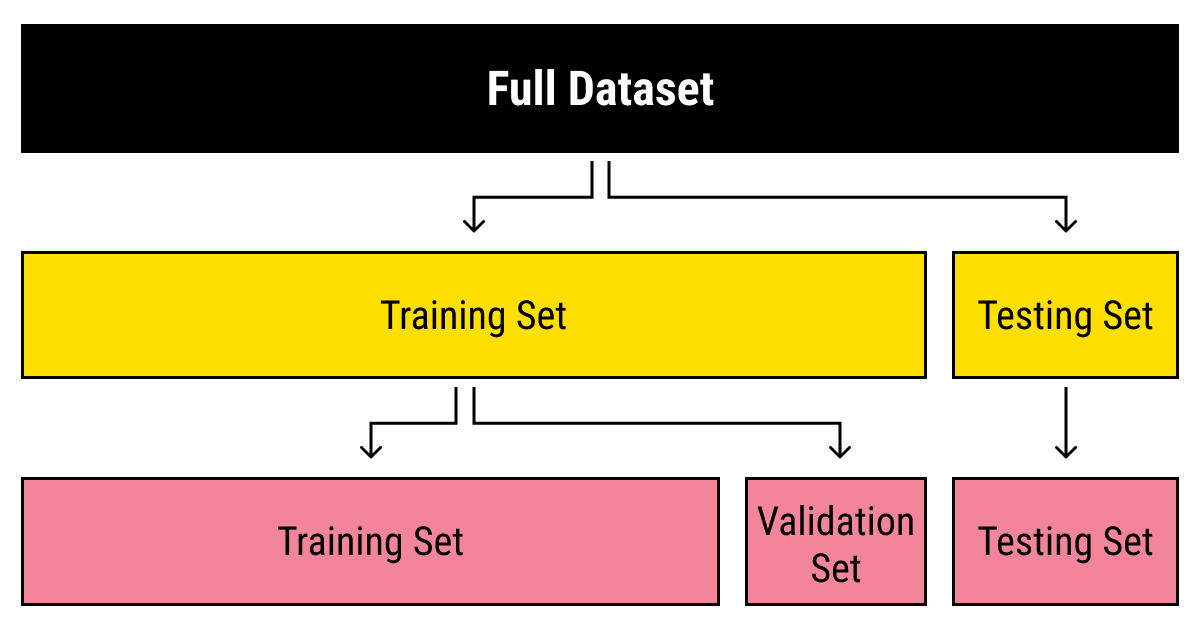
\includegraphics[width=\linewidth]{./img/particion.png}
    		\caption{Partición de los datos para cada fase del desarrollo del modelo.}
	\end{figure}

\end{frame}

%\subsection{Características de los datos}
%\begin{frame}{Origen de los datos}

%\begin{itemize}
%	\item El dataset utilizado en este trabajo es \texttt{NF-UNSW-NB15-v3}, desarrollado como parte de un análisis realizado en la Universidad de Queensland, Australia.
%	 \vspace{10mm}
%	\item Contiene 53 atributos que describen características del tráfico de red y que permiten clasificar las muestras de tráfico en nueve clases de ataques o como conexiones benignas. 
%	 \vspace{10mm}
%	\item Algunos de los datos que recoge, son:
%\begin{itemize}
%	\item La duración de la conexión.
%	\item Los bytes enviados y los recibidos.
%	\item Versiones de los protocolos utilizados.
%\end{itemize}

%\end{itemize}
%\end{frame}

%\begin{frame}{Tipos de ataques registrados en el conjunto de datos}

%\begin{table}[H]
%\centering
%\begin{tabular}{|c|r|} 
%\hline
%\rowcolor[HTML]{f0f7ff}  
%\textbf{Clase} & \textbf{Cantidad} \\ \hline
%Benigno & 2\,237\,731 \\ \hline
%\textit{Fuzzers} & 33\,816 \\ \hline
%\textit{Analysis} & 2\,381 \\ \hline
%\textit{Backdoor} & 1\,226 \\ \hline
%DoS & 5\,980 \\ \hline
%\textit{Exploits} & 42\,748 \\ \hline
%\textit{Generic} & 19\,651 \\ \hline
%\textit{Reconnaissance} & 17\,074 \\ \hline
%\textit{Shellcode} & 4\,659 \\ \hline
%\textit{Worms} & 158 \\ \hline
%\end{tabular}
%\caption{Clasificación de amenazas de seguridad del \textit{dataset} %\texttt{NF-UNSW- NB15-v3}.}
%\label{tab:attacks-tab}
%\end{table}

%\end{frame}

%\subsection{Preparación de los datos}

%\begin{frame}{Atributos}
%	Los atributos utilizados para desarrollar los modelos de este trabajo son los 53 atributos del conjunto de datos original, excepto los siguientes que han sido eliminados:
%	\begin{itemize}
%		\item \texttt{IPV4\_SRC\_ADDR}
%		\item \texttt{IPV4\_DST\_ADDR}
%		\item \texttt{FLOW\_START\_MILLISECONDS}
%		\item \texttt{FLOW\_END\_MILLISECONDS}
%	\end{itemize}
%\end{frame}

%\begin{frame}{Etiquetas}
%	\begin{itemize}
	
%		\item \texttt{Label}: Indica si se trata de una conexión benigna o maligna.
%		 \vspace{10mm}
%		\item \texttt{Attack}: Indica el tipo de ataque al que corresponde esa conexión.
%	\end{itemize}
%\end{frame}

